%Para este capítulo se usará la abreviatura "conex".
\chapter{Conexión}
\label{conex}

La noción de conexión es otra más de las nociones que ya conocíamos en $\R^n$ que pueden generalizarse a un espacio topológico arbitrario. Un conjunto es, intuitivamente, conexo, si está hecho ``de una sola pieza''. 

\section{Definición y propiedades}

Empezaremos viendo, por supuesto, la definición, y una serie de caracterizaciones equivalentes.

\begin{defi}[Conexión]
	Un espacio topológico $\X$ es \tbi[espacio!conexo|see{conexo}]{conexo} \indexg{conexo} si no es unión de dos abiertos disjuntos no vacíos, esto es, no existen $U,V\neq\emptyset$, abiertos, tales que $U\cap V=\emptyset$ y $X=U\cup V$.
\end{defi}

\begin{obs}[Conexión en subespacios]
	De nuevo, como con compacidad, la conexión en un subconjunto no necesita una definición alternativa. Dado $\mc{Y}\subset\X$, simplemente decimos que $\mc{Y}$ es conexo si lo es entendido como espacio equipado con la topología relativa. Nótese que esta definición es equivalente a la mucho más rebuscada que dábamos en $\R^n$, que involucraba abiertos relativos.
\end{obs}

\begin{prop}[Definiciones equivalentes de conexión]
	Sea un espacio topológico $\X$. Las siguientes afirmaciones son equivalentes:
	\begin{enumerate}
		\item $\X$ es conexo.
		\item $\X$ no es unión de dos cerrados disjuntos no vacíos, esto es, no existen $F,G\neq\emptyset$, cerrados, tales que $F\cap G=\emptyset$ y $X=F\cup G$.
		\item No hay ningún conjunto abierto y cerrado no trivial, esto es, $\nexists U$ abierto y cerrado tal que $U\neq\emptyset$ y $U\neq\X$.
	\end{enumerate}
\end{prop}

Es inmediato, y se deja al lector, comprobar estas equivalencias.

\begin{exa}
	En $\R$, los conexos son los intervalos. En efecto, si $A\subset\R$ no es un intervalo, entonces por definición $\exists a\notin A$ tal que $\inf A< a < \sup A$. Entonces, $(-\infty, a)\cap A$ y $(a,\infty)\cap A$ son dos abiertos disjuntos no vacíos cuya unión contiene a $A$.
\end{exa}

Ahora, vamos a repasar brevemente las propiedades que ya conocíamos de conjuntos conexos.

\begin{prop}[Imagen continua]
	\label{conex_prop_im_continua}
	La imagen continua de un conexo es un conexo.
\end{prop}
\begin{proof}
	Sea $\X$ conexo, $f:\X\to\Y=f(\X)$ continua. Entonces queremos ver que $\mc{Y}$ es conexo. Para ello vamos a ver el contrarrecíproco: si $\Y$ no es conexo $\X$ tampoco.
	
	Al no ser $\Y$ conexo, existe $A\subset\Y$ abierto y cerrado no trivial (esto es, que no es ni el vacío ni el total). Entonces por ser $f$ continua, $f^{-1}(A)$ es también abierto y cerrado, y por ser $f$ sobreyectiva $f^{-1}(A)$ no es el vacío ni el total. Por tanto $\X$ no es conexo.
\end{proof}

% NOTA: no he nombrado el teorema como teorema del pivote porque buscado en internet sólo salía en la página de Ruiz con ese nombre. En demás libros que he visto no tiene nombre.

A continuación presentamos un teorema conocido en algunos lugares remotos como el teorema del pivote.

\begin{theo}
	\label{conex_theo_pivote}
	Sea $\{A_i\}_{i\in I}$ una familia de conexos de $\X$ tales que existe $a\in\bigcap_{i\in I} A_i$. Entonces $\bigcup_{i\in I} A_i$ es conexo.
\end{theo}
\begin{proof}
	Supongamos que existe $S\subset\bigcup_{i\in I} A_i$ abierto y cerrado de la unión. Vamos a ver que necesariamente es el vacío o el total.
	
	Para cada $i\in I$ tenemos que $S\cap A_i\subset A_i$ es abierto y cerrado en $A_i$. Ahora, como $A_i$ es conexo, $S\cap A_i$ tiene que ser necesariamente el vacío o el total, para cada $i\in I$. Distinguimos pues dos casos:
	\begin{enumerate}
		\item Si $S\cap A_i=\emptyset$ para todo $i\in I$, entonces $S=\emptyset$ y ya está.
		\item Si $\exists i_0\in I$ tal que $S\cap A_{i_0}=A_{i_0}$, entonces, como $a$ está en la intersección de la familia, en particular $a\in A_{i_0}= S\cap A_{i_0}$ y, por tanto, $a\in S$. Esto implica que $a\in S\cap A_i$ para todo $i\in I$, con lo que ninguno de los $S\cap A_i$ es vacío. Como necesariamente deben ser el vacío o el total, $S\cap A_i=A_i$ para todo $i\in I$. Con ello, $A_i=S\cap A_i\subset S$ para todo $i\in I$, lo cual implica que $\bigcup_{i\in I} A_i\subset S$. Es decir, $S=\bigcup_{i\in I} A_i$, con lo que hemos terminado.
	\end{enumerate}
\end{proof}

Este teorema es extremadamente útil para garantizar la conexión de un sinnúmero de conjuntos, y genera un gran abanico de corolarios y consecuencias. Aquí vamos a detallar algunos que se usan con frecuencia.

\begin{cor}
	\label{conex_cor_pivote_corte_comun}
	Sea $\{A_i\}_{i\in I}$ una familia de conexos que cumple que $\exists i_0\in I$ tal que $A_{i_0}\cap A_i\neq\emptyset\;\;\forall i\in I$. Entonces $\bigcup_{i\in I} A_i$ es conexo. En particular, el resultado se verifica si la familia cumple que $A_i\cap A_j\neq\emptyset\;\;\forall i\neq j$.
	
	\begin{proof}
		Como $A_i\cap A_{i_0}\neq\emptyset$ por hipótesis, podemos aplicar el teorema \ref{conex_theo_pivote} para cada $i\in I$, y por tanto cada $A_{i_0}\cup A_i$ es conexo. Ahora, escribimos:
		\[\bigcup_{i\in I} A_i = \bigcup_{i\in I} (A_i\cup A_{i_0})\]
		y como todos comparten los elementos de $A_{i_0}$, podemos aplicar el teorema de nuevo.
	\end{proof}
\end{cor}

\begin{cor}
	Sea una cadena $\{A_i\}_{i=1}^n$ de conexos que verifica que $A_i\cap A_{i+1}\neq\emptyset$. Entonces $\bigcup_{i=1}^n A_i$ es conexo.
	
	\begin{proof}
		Por inducción, se aplica el teorema \ref{conex_theo_pivote} a $A_1\cup A_2$, $(A_1\cup A_2)\cup A_3$, ..., $\left(\bigcup_{i=1}^k A_i\right)\cup A_{k+1}$.
	\end{proof}
\end{cor}

\begin{obs}
	El corolario anterior también se verifica si la sucesión de conjuntos es numerable, pero no lo vamos a probar aquí.
	% AQUÍ VIENE PROBADO http://dbfin.com/topology/munkres/chapter-3/section-23-connected-spaces/problem-2-solution/
\end{obs}

El siguiente resultado, aunque también es consecuencia del teorema \ref{conex_theo_pivote}, es más que un mero corolario y merece la categoría de teorema por sí mismo.

\begin{theo}\label{T7:teo_adherencia_conexa}
	Sea $A$ conexo y $B$ tal que $A\subset B\subset\adher{A}$. Entonces $B$ es conexo. En particular $\adher{A}$ es conexo.
	
	\begin{proof}
		Como podemos escribir:
		\[B=\bigcup_{b\in B\setminus A} (A\cup\{b\}) \]
		y todos comparten un punto, entonces basta probar que cada $A\cup\{b\}\subset\adher{A}$ es conexo, pues en ese caso el teorema \ref{conex_theo_pivote} nos garantiza la conexión de $B$.
		
		Supongamos que $\exists C\subset A\cup\{b\}$ abierto y cerrado y no trivial. Entonces, $C\cap A\subset A$ y es abierto y cerrado en $A$. Como $A$ es conexo distinguimos dos casos:
		
		\begin{itemize}
			\item Si $C\cap A=\emptyset$, entonces $C=\{b\}$ y por tanto $\{b\}$ es abierto, luego, como el entorno $\{b\}$ de sí mismo no corta con $A$, $b\notin\adher{A}$, lo cual es una contradicción.
			\item Si $C\cap A=A$, $C=A$ y por tanto $A$ es cerrado, pero $b\notin A=\adher{A}$, que de nuevo es una contradicción. \qedhere
		\end{itemize}
	\end{proof}
\end{theo}

Aprovechando los resultados anteriores podemos garantizar la conexión de un buen número de espacios.

\begin{exa} Veamos algunos ejemplos de conjuntos conexos:
	\begin{enumerate}
		\item En $\R^n$, se dice que un conjunto es \tbi{convexo} si para cada par de puntos el segmento que los une también está en el conjunto; y se dice que es \tbi{estrellado} si existe un punto tal que el segmento de él a cualquier otro está en el conjunto. Si un conjunto es convexo entonces es estrellado, y si es estrellado entonces es conexo. Además, las implicaciones recíprocas no se verifican.
		\[\text{Convexo}\ra\text{Estrellado}\ra \text{Conexo}\]
		
		En efecto, un conjunto $A$ estrellado se puede escribir como:
		\[A=\bigcup_{a\in A} [a_0, a]\]
		para cierto $a_0\in A$. Cada segmento $[a_0,a]$ es conexo por la proposición \ref{conex_prop_im_continua}, al ser la imagen del intervalo conexo $[0,1]$ por la aplicación:
		\[t\mapsto (1-t)a_0+ta\]
		y por tanto, por el teorema \ref{conex_theo_pivote}, como todos comparten el punto $a_0$, su unión es conexa.
		
		Nótese que ni la convexidad ni ser estrellado son propiedades topológicas; ambas son propiedades métricas: su definición solo tiene sentido en un espacio que, al menos, tenga definida una distancia.
		
		\item Una circunferencia en $\R^2$ es conexa, pero no es estrellada. En efecto, es conexa por ser la imagen de $[0,2\pi]$ por la aplicación $t\mapsto (\cos t, \sen t)$.
		
		\item El grafo de la función $\sin\frac{1}{x}$ para $x>0$, que escribimos:
		\[C = \left\{\left(x,\sin\frac{1}{x}\right)\midc x>0\right\}\]
		es conexo por ser la imagen continua de $(0,\infty)$ por la aplicación:
		\[x\mapsto \left(x,\sin\frac{1}{x}\right)\]
		
		Lo que es más interesante, para cualquier $a\in [-1,1]$ se verifica que $\{(0,a)\}$ es adherente a $C$ y por tanto que $C\cup\{(0,a)\}$ es conexo.
		\begin{figure}[H]
			\centering
			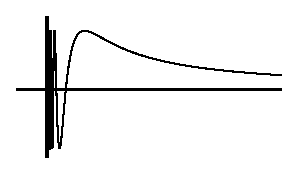
\includegraphics[scale = 1.3]{img/funcionsen1x}
		\end{figure}
		
		\item Consideramos el conjunto:
		\[C = \big(\{0\}\times (0,1]\big) \cup \left(\bigcup_{n\in\N} [0,1]\times\left\{\frac{1}{n}\right\}\right) \]
		que es unión de segmentos horizontales cada vez más juntos y de un segmento vertical. Este es trivialmente conexo por el corolario \ref{conex_cor_pivote_corte_comun}. Lo particular es que si unimos a $C$ el segmento horizontal:
		\[(0,1)\times\{0\}\]
		sigue siendo conexo por ser adherencia de $C$. 
		\begin{figure}[H]
			\centering
			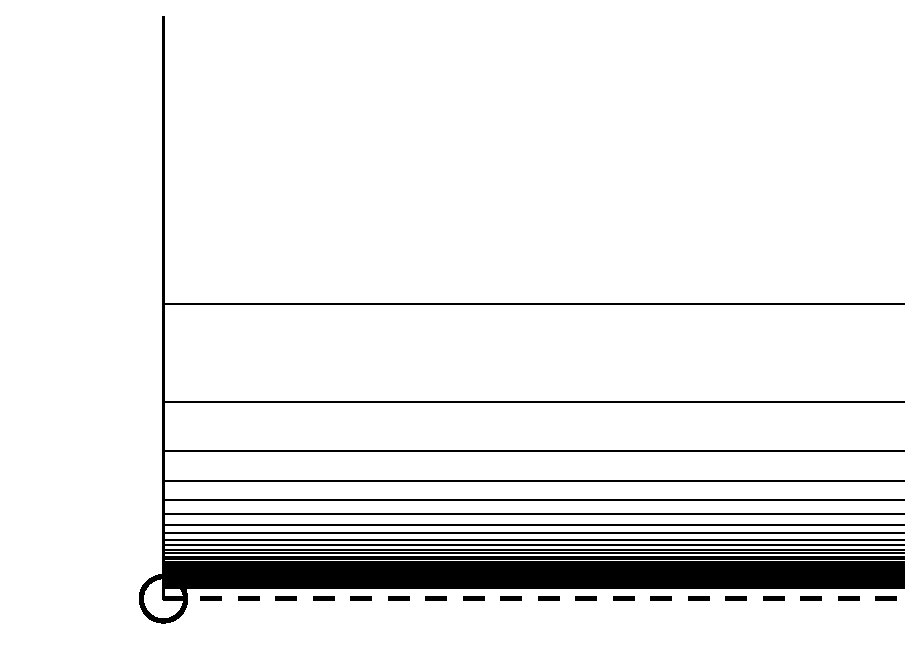
\includegraphics[scale = 2.5]{img/lineas}
		\end{figure}
	\end{enumerate}
\end{exa}

Completamos esta sección con una propiedad interesante garantizada por la conexión.

\begin{lem}
	Sea $\X$ conexo y $\{U_i\}_{i\in I}$ una familia de abiertos, de forma que $\X=\bigcup_{i\in I} U_i$. Dos puntos cualesquiera $x,y\in\X$ se pueden conectar mediante una cadena finita $\{U_{i_k}\}_{k=1}^n$ de abiertos de la familia que verifique que $U_{i_k}\cap U_{i_{k+1}}\neq\emptyset$.
	
	\begin{proof}
		Sea $A=\{z\in\X \midc \text{existe una cadena de } x \text{ a } z \}$. $A$ es claramente no vacío, puesto que $x\in A$. Entonces, una forma de ver que $\X=A$, que es lo que queremos encontrar, es comprobar que $A$ es abierto y cerrado, puesto que entonces solo puede ser el total (pues hemos visto que es no vacío y $\X$ es conexo).
		
		\begin{itemize}
			\item Veamos que $A$ es abierto. En efecto, dado $z\in A$, queremos ver que existe un abierto $U$ tal que $z\in U\subset A$. Pero basta con tomar el último de la cadena, que ya cumple estas condiciones.
			
			\item Ahora veamos que es cerrado. En efecto, si $z\in\adher{A}$, existe un abierto $U_{i_0}$ tal que $U_{i_0}\cap A\neq\emptyset$. Entonces, tomamos un punto $y$ de la intersección, y como está en $A$ hay una cadena de $x$ a $y$. Uniendo $U_{i_0}$ a la cadena tenemos una cadena de $x$ a $z$, y por tanto $z\in A$, luego $A=\adher{A}$. \qedhere
		\end{itemize}
	\end{proof}
\end{lem}

\begin{obs}
	En particular, puedo recubrir cualquier abierto conexo de $\R^n$ por bolas, y por tanto existe una cadena de bolas que une cualquier par de puntos. Si tomo un punto en cada intersección entre bolas consecutivas de la cadena y los uno, tengo una poligonal que conecta los dos puntos. Entonces, si $C\subset\R^n$ es abierto, $C$ es conexo si y solo si es conexo por poligonales (la definición de conexión por poligonales y la implicación inversa corresponden a cálculo diferencial).
\end{obs}

\section{Componentes conexas}

Al igual que ocurría con la compacidad, sería deseable que todos los espacios fuesen conexos. Dado que esto no se da, nos conformaremos con quedarnos con los subconjuntos conexos del espacio. Surge así la idea de componente conexa que definimos a continuación. Aunque parezca que esto no es una ventaja, es tremendamente útil a la hora de estudiar, por ejemplo, si dos espacios son homeomorfos.

\begin{defi}
	Un subconjunto $\Co\subset\X$ es una \tbi{componente conexa} si es un conjunto conexo maximal.
\end{defi}

Una consecuencia inmediata de la definición es que, dado $x\in\X$,
\begin{equation}
	\Co(x)=\bigcup_{x\in A \text{ conexo}} A
\end{equation}
es una componente conexa, que denominaremos componente conexa de $x$.

En efecto, la unión no es vacía, pues el punto en sí es conexo. Además $x$ pertenece a la intersección de todos ellos. Como cada $A$ es conexo, basta aplicar el teorema del pivote para deducir que $\Co(x)$ es conexo. Por construcción es, además, maximal, ya que cualquier conexo que lo contenga, contiene a $x$ y, por tanto, está en la unión.

Cabe destacar que $\Co(x)$ es más que maximal, ya que cumple lo siguiente. Sea $E\subset\X$ conexo tal que $E\cap \Co(x)\not=\emptyset$. Entonces $E\cup \Co(x)$ es conexo y además $x\in E\cup \Co(x)$, por lo que $E\cup \Co(x)\subset \Co(x)$, es decir, $E\subset \Co(x)$.

Esto será muy utilizado de aquí en adelante, cualquier conexo que interseque con una componente conexa está contenido en ella.

\begin{obs}
	Nótese que hay varios punto con la misma componente conexa y que si el espacio es conexo, entonces es la componente conexa de todos los puntos.
\end{obs}

A continuación enunciamos y demostramos algunas propiedades de las componentes conexas.

\begin{lem}
	Sea $\X$ un espacio topológico, entonces:
	\begin{enumerate}
		\item Las componentes conexas son cerradas.
		
		\item Las componentes conexas son una partición del espacio.
		
		\item Si $\X$ es la unión disjunta de las componentes conexas, siendo estas finitas, entonces las componentes conexas son abiertas.
		
		\item Si en $\X$ todo punto tiene un entorno conexo, entonces las componentes conexas de $\X$ son abiertas.
	\end{enumerate}
\end{lem}
\begin{proof}
	Vayamos con la demostración:
	\begin{enumerate}
		\item Sea $\Co(x)$ componente conexa. Como es conexo, por el teorema~\ref{T7:teo_adherencia_conexa} su adherencia es conexa, y por ser maximal $\Co(x)=\adher{\Co(x)}$.
		
		\item Es claro que
		\[\X=\bigcup_{x\in\X} \Co(x)\]
		Además, dadas dos componentes conexas, $\Co_1$ y $\Co_2$, si $\Co_1\cap\Co_2\not=\emptyset$ entonces $\Co_1\subseteq\Co_2$ y por ser maximales se da la igualdad.
		
		\item Por hipótesis $\X=\Co_1\cup\cdots\cup\Co_r$ siendo la unión disjunta. Entonces, para cada $i\in\{1,\cdots r\}$ se tiene que 
		\[\Co_i=\X\backslash (\Co_1\cup\cdots\cup\Co_{i-1}\cup\Co_{i+1}\cup\cdots\cup\Co_r)=\X\backslash \Co\]
		Como cada componente conexa es cerrada por 1, la unión finita es cerrada $\Co$, luego $C_i=\X\backslash \Co$ es abierto para todo $i$.
		
		\item Sea $\Co$ componente conexa de $\X$ y veamos que es entorno de todos sus puntos. Sea $x\in\Co$. Por hipótesis existe $\V$ entorno conexo de $x$, con lo cual $\V\cap\Co\not=\emptyset$. Esto implica que $x\in\V\subset\Co$, con lo que $\Co$ es entorno de $x$.
	\end{enumerate}
\end{proof}

%Tablas comportamiento topológico. Añado aquí también las de conexión por caminos, dado que no está aun el tema.

\section{Comportamiento topológico}

\begin{table}[h]
	\centering
	\begin{tabular}{l|l|l|l|l|}
		\cline{2-5}
		& \textbf{Subespacios}    & \textbf{Cociente}       & \textbf{Producto}       & \textbf{Suma}           \\ \hline
		\multicolumn{1}{|c|}{\textbf{Conexión}} & \multicolumn{1}{c|}{No} & \multicolumn{1}{c|}{Sí*} & \multicolumn{1}{c|}{Sí} & \multicolumn{1}{c|}{No} \\ \hline
	\end{tabular}
	\caption{Tabla resumen de conexión.}
	\label{Tabla_conexion}
\end{table}

\begin{table}[h]
	\centering
	\begin{tabular}{l|l|l|l|l|}
		\cline{2-5}
		& \textbf{Subespacios}                                                                      & \textbf{Cociente}       & \textbf{Producto}       & \textbf{Suma}           \\ \hline
		\multicolumn{1}{|c|}{\textbf{\begin{tabular}[c]{@{}c@{}}Local\\ conexión\end{tabular}}} & \multicolumn{1}{c|}{\begin{tabular}[c]{@{}c@{}}Sí, en el caso\\ de abiertos\end{tabular}} & \multicolumn{1}{c|}{Sí} & \multicolumn{1}{c|}{Sí} & \multicolumn{1}{c|}{Sí} \\ \hline
	\end{tabular}
	\caption{Tabla resumen de local conexión}
	\label{Tabla_localconexion}
\end{table}

\begin{table}[h]
	\centering
	\begin{tabular}{c|c|c|c|c|}
		\cline{2-5}
		\multicolumn{1}{l|}{}                                                                                  & \multicolumn{1}{l|}{\textbf{Subespacios}}                             & \multicolumn{1}{l|}{\textbf{Cociente}} & \multicolumn{1}{l|}{\textbf{Producto}} & \multicolumn{1}{l|}{\textbf{Suma}} \\ \hline
		\multicolumn{1}{|c|}{\textbf{\begin{tabular}[c]{@{}c@{}}Conexo por\\ caminos\end{tabular}}}            & No                                                                    & Sí                                     & Sí                                     & No                                 \\ \hline
		\multicolumn{1}{|c|}{\textbf{\begin{tabular}[c]{@{}c@{}}Localmente conexo\\ por caminos\end{tabular}}} & \begin{tabular}[c]{@{}c@{}}Sí, en el caso \\ de abiertos\end{tabular} & Sí                                     & Sí                                     & Sí                                 \\ \hline
	\end{tabular}
	\caption{Tabla resumen de conexión por caminos}
	\label{Tabla_conexion_caminos}
\end{table}

\begin{figure}[h!]
	\centering
	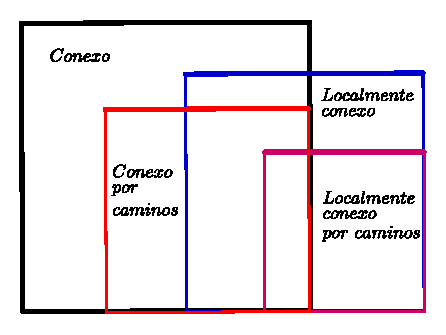
\includegraphics[scale = 1]{img/Comparacion_conexion}
\end{figure}
